\subsection{Pressione}

Variamo la pressione nella camera tenendo la sorgente a \SI{0}{\degree} per cercare in quali condizioni l'aria residua non influisce sulla misura.
Registriamo per ogni valore della pressione il rate di eventi ed il relativo spettro. In \autoref{tab:press} sono presenti i dati ed in \autoref{fig:press} il loro andamento.

\marginpar{qui mi riferisco agli angoli segnati sulla scala graduata, ricordiamoci che gli angoli rispetto al fotodiodo sono altri}

\marginpar{aggiungere gli errori delle mode}

\begin{table}[h]
\centering
\begin{tabular}{|c|c|c|}
\hline
pressione [mbar] & rate [\si{s^{-1}}] & moda [digit] \\
\hline
$ 0.0190 \pm 0.0010 $ & $ 44.6 \pm 0.9 $ & $ 3183 $ \\ 
$ 0.180 \pm 0.010 $ & $ 46.4 \pm 1.0 $ & $ 3182 $ \\ 
$ 1.00 \pm 0.20 $ & $ 44.8 \pm 0.9 $ & $ 3181 $ \\ 
$ 8.90 \pm 0.10 $ & $ 45.4 \pm 0.8 $ & $ 3172 $ \\ 
$ 23.0 \pm 1.0 $ & $ 44.9 \pm 0.9 $ & $ 3153 $ \\ 
$ 63.0 \pm 1.0 $ & $ 43.1 \pm 0.8 $ & $ 3103 $ \\ 
$ 81.0 \pm 1.0 $ & $ 44.0 \pm 0.7 $ & $ 3078 $ \\ 
$ 110 \pm 10 $ & $ 47.1 \pm 1.0 $ & $ 3049 $ \\ 
$ 150 \pm 10 $ & $ 44.4 \pm 0.9 $ & $ 3027 $ \\ 
$ 220 \pm 10 $ & $ 43.4 \pm 0.8 $ & $ 2984 $ \\ 
$ 470 \pm 10 $ & $ 45.9 \pm 0.9 $ & $ 2787 $ \\ 
$ 700 \pm 10 $ & $ 41.7 \pm 0.9 $ & $ 1712 $ \\ 
$ 860 \pm 10 $ & $ 0.13 \pm 0.04 $ & $ 521 $ \\ 
\hline
\end{tabular}
\caption{Dati per stimare l'effetto della pressione sulle misure. L'errore sulla moda è dato dall'intervallo di credibilità del 90\% calcolato sul relativo istogramma.}
\label{tab:press}
\end{table}

Dal grafico di \autoref{fig:press} non si nota nessuna variazione dei conteggi fino ad \SI{1}{atm}, ma la moda dello spettro inizia a decrescere quando la pressione è maggiore di \SI{200}{mbar}. 
Come atteso, la distribuzione di energia persa dalle particelle $\alpha$ in aria diventa sempre più larga all'aumentare della pressione.
Questo risultato ci assicura una grande indipendenza dalla condizione di vuoto della camera, soprattutto durante le misure notturne. In tale periodo della giornata è vietato tenere la pompa accesa e, come abbiamo potuto verificare, la pressione risale fino al mbar anche dopo due giorni dalla chiusura della pompa. Quindi possiamo tranquillamente fare misure di lunga durata.

\begin{figure}[h]
\centering
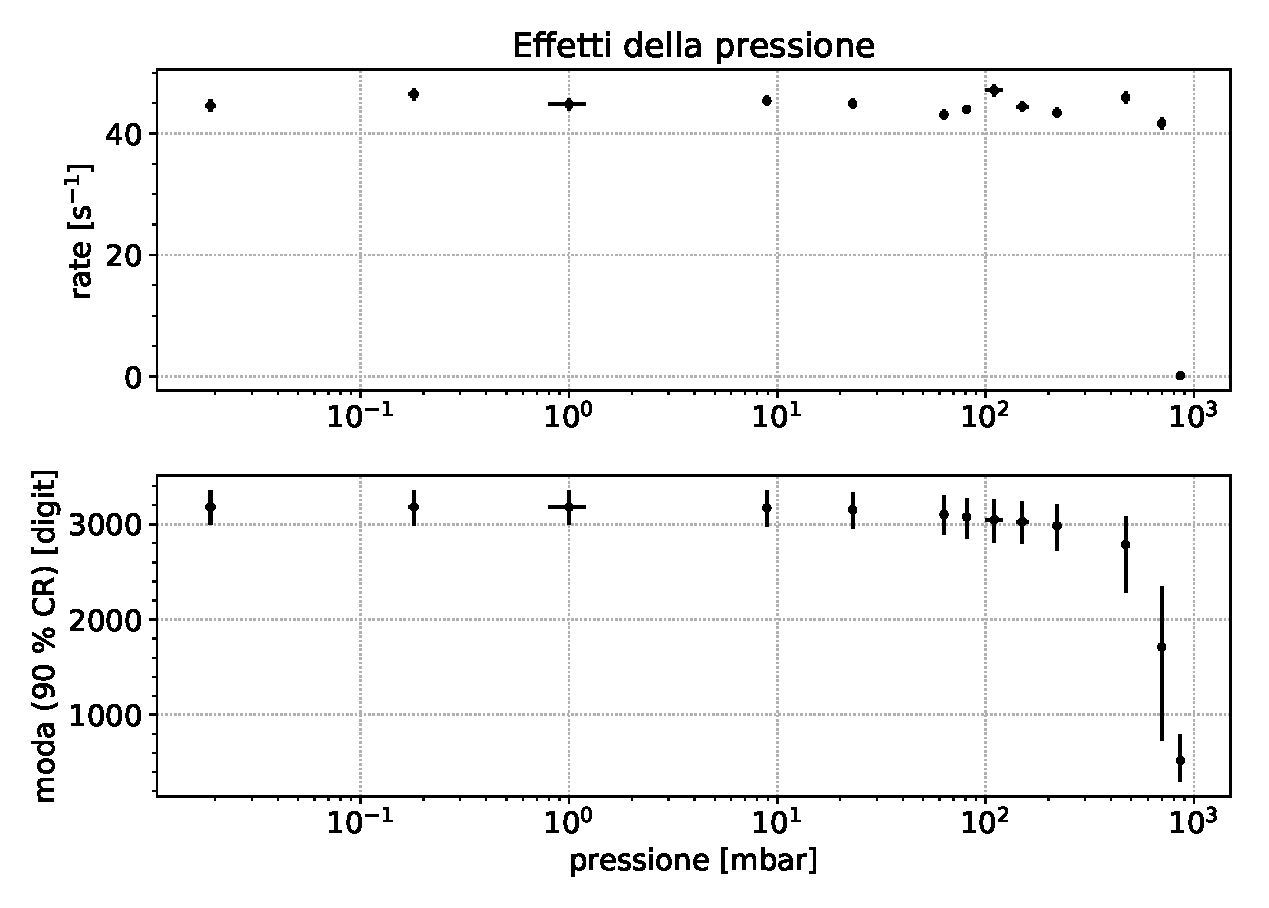
\includegraphics[width=30 em]{immagini/press}
\caption{Effetti della pressione su conteggi e spettri. Il pannello superiore mostra il variare del rate al variare la pressione, quello sottostante contiene la moda dei relativi spettri con errore un intervallo del 90\% di credibilità.}
\label{fig:press}
\end{figure}



\marginpar{secondo me dobbiamo mostrare questa cosa con l'istogramma di alcuni spettri perché dà un'idea più immediata rispetto al fornire l'intervallo di credibilità}

